\graphicspath{{chapt_dutch/}{intro/}{chapt2/}{chapt3/}{chapt4/}{chapt5/}{chapt6/}{chapt7/}}

% Header
\renewcommand\evenpagerightmark{{\scshape\small Chapter 2}}
\renewcommand\oddpageleftmark{{\scshape\small Investigating the\si{TeV} scale}}

\renewcommand{\bibname}{References}

\hyphenation{}

\chapter[Investigating the\si{TeV} scale]%
{Investigating the\si{TeV} scale}
\label{chap:2}

\section{The Standard Model of Particle Physics}
\label{sec:SM}

\section{The \acl{LHC} and the \acl{CMS}}
\label{sec:LHC-CMS}

\section{Muon Phase-II Upgrade}
\label{sec:phase-2}

After the more than two years lasting \acf{LS1}, the \acf{LHC} delivered its very first Run-II proton-proton collisions early 2015. LS1 gave the opportunity to the LHC and to the its experiments to undergo upgrades. The accelerator is now providing collisions at center-of-mass energy of \SI{13}{TeV} and bunch crossing rate of \SI{40}{MHz}, with a peak luminosity exceeding its design value. During the first and upcoming second LHC Long Shutdown, the \acf{CMS} detector is also undergoing a number of upgrades to maintain a high system performance~\cite{MUONTDR}.

From the LHC Phase-2 or \acf{HL-LHC} period onwards, i.e. past the \acf{LS3}, the performance degradation due to integrated radiation as well as the average number of inelastic collisions per bunch crossing, or pileup, will rise substantially and become a major challenge for the LHC experiments, like CMS that are forced to address an upgrade program for Phase-II~\cite{PHASEIITP}. Simulations of the expected distribution of absorbed dose in the CMS detector under HL-LHC conditions, show in figure~\ref{fig:Dose} that detectors placed close to the beamline will have to withstand high irradiation, the radiation dose being of the order of a few tens of\si{Gy}.

\begin{figure}[ht!]
	\centering
	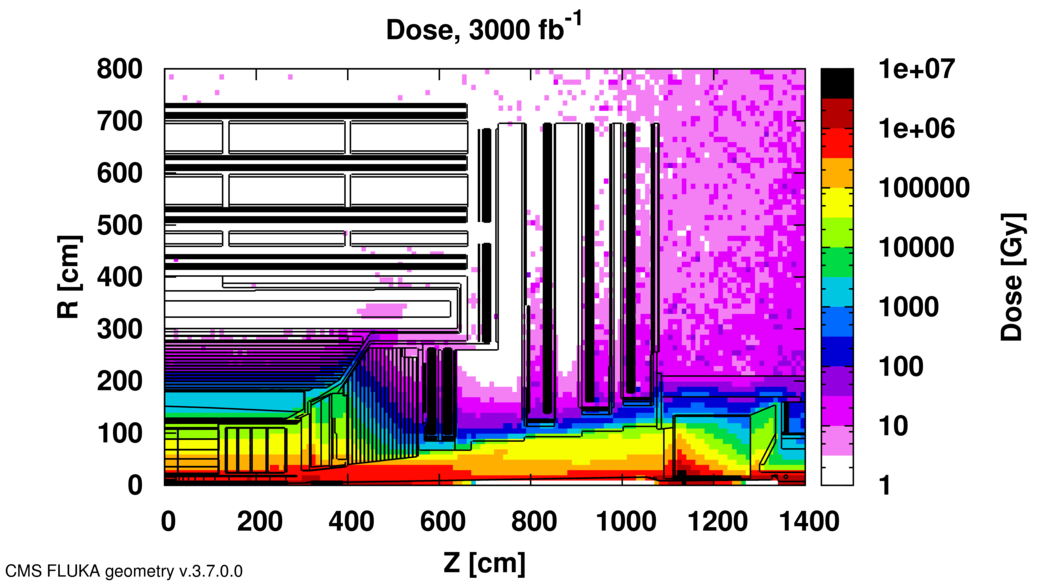
\includegraphics[width=0.7\textwidth]{fig/HL-LHC-Dose.png}
	\caption{\label{fig:Dose} Absorbed dose in the CMS cavern after an integrated luminosity of \SI{3000}{\femto\per\barn}. R is the transverse distance from the beamline and Z is the distance along the beamline from the Interaction Point at Z=0.}
\end{figure}

The measurement of small production cross-section and/or decay branching ratio processes, such as the Higgs boson coupling to charge leptons or the $B_s \longrightarrow \mu^+\mu^-$ decay, is of major interest and specific upgrades in the forward regions of the detector will be required to maximize the physics acceptance on the largest possible solid angle. To ensure proper trigger performance within the present coverage, the muon system will be completed with new chambers. In figure~\ref{fig:Quadrant} one can see that the existing \acfp{CSC} will be completed by \acfp{GEM} and \acfp{RPC} in the pseudo-rapidity region $1.6<\vert\eta\vert<2.4$ to complete its redundancy as originally scheduled in the CMS Technical Proposal~\cite{CMSTP}.

\begin{figure}[ht!]
	\centering
	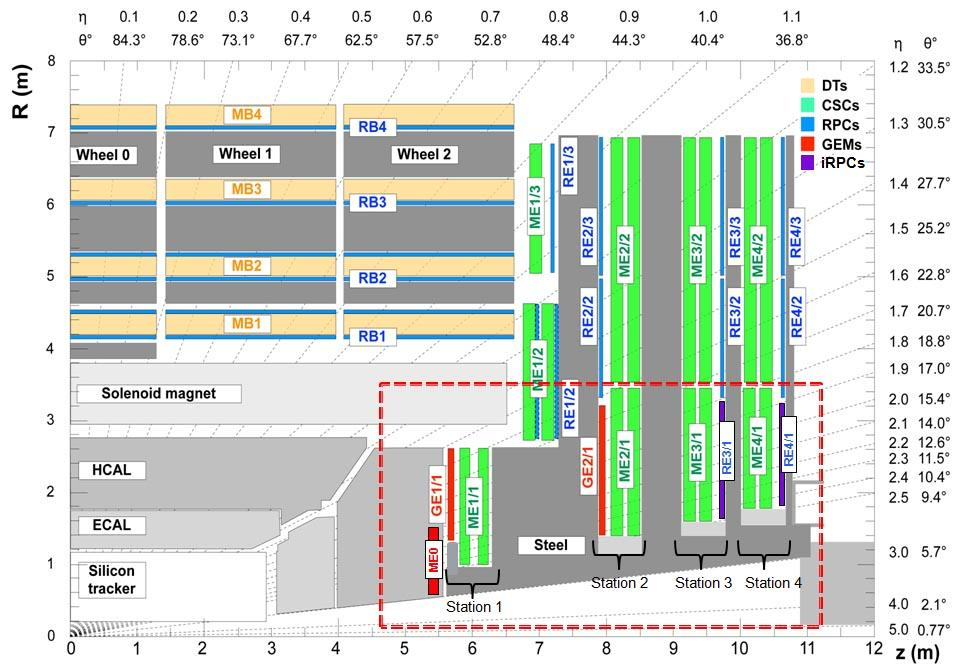
\includegraphics[width=0.7\textwidth]{fig/MuonUpgrade-Plans.jpg}
	\caption{\label{fig:Quadrant} A quadrant of the muon system, showing DTs (yellow), RPCs (light blue), and CSCs (green). The locations of new forward muon detectors for Phase-II are contained within the dashed box and indicated in red for GEM stations (ME0, GE1/1, and GE2/1) and dark blue for improved RPC (iRPC) stations (RE3/1 and RE4/1).}
\end{figure}

RPCs are used by the CMS first level trigger for their good timing performances. Indeed, a very good bunch crossing identification can be obtained with the present CMS RPC system, given their fast response of the order of \SI{1}{ns}. In order to contribute to the precision of muon momentum measurements, muon chambers should have a spatial resolution less or comparable to the contribution of multiple scattering~\cite{MUONTDR}. Most of the plausible physics is covered only considering muons with $p_T<$\SI{100}{GeV} thus, in order to match CMS requirements, a spatial resolution of $\mathcal{O}$(few $\mathrm{mm}$) the proposed new RPC stations, as shown by the simulation in figure~\ref{fig:MultiScat}. According to preliminary designs, RE3/1 and RE4/1 readout pitch will be comprised between 3 and \SI{6}{mm} and 5 $\eta$-partitions could be considered.

\begin{figure}[ht!]
	\centering
	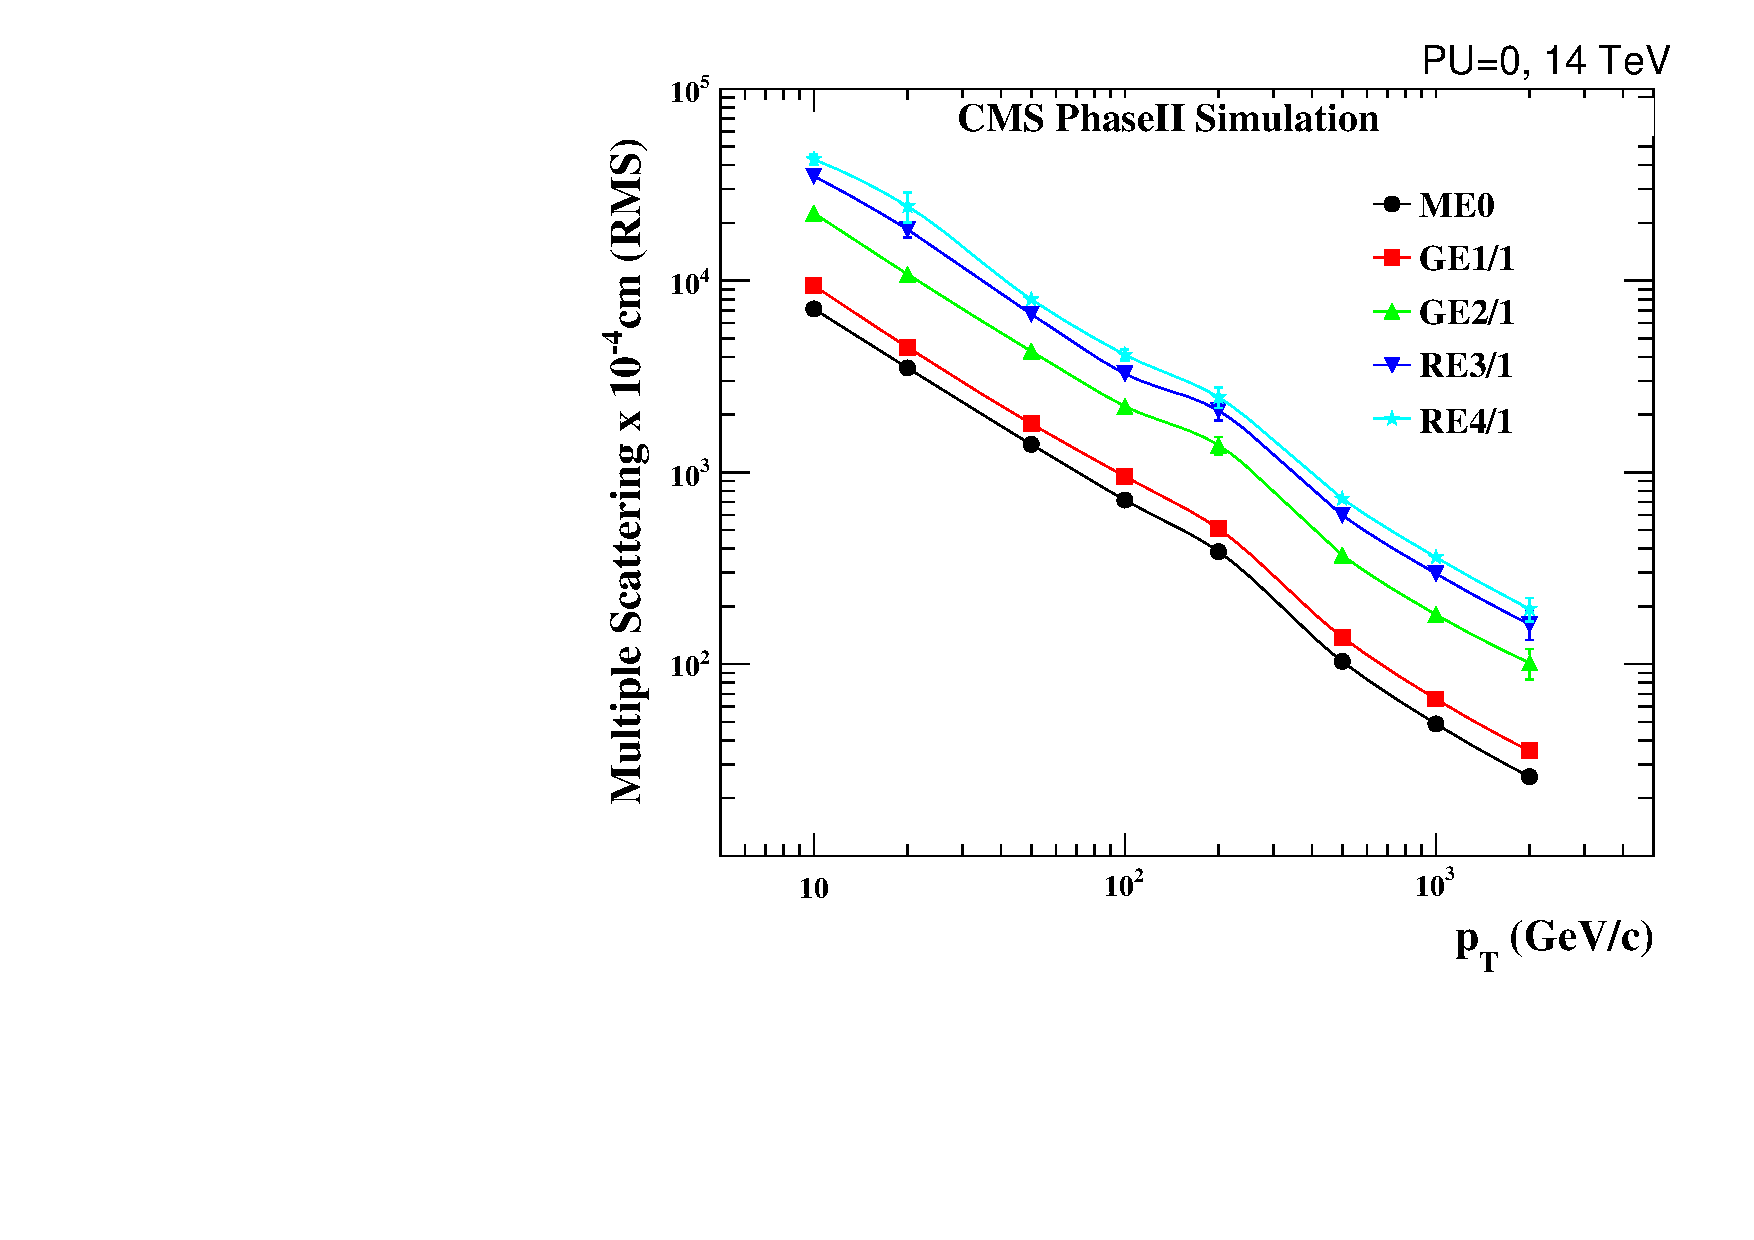
\includegraphics[width=0.6\textwidth]{fig/MS_allstations.pdf}
	\caption{\label{fig:MultiScat}  RMS of the multiple scattering displacement as a function of muon $p_T$ for the  proposed forward muon stations. All of the electromagnetic processes such as bremsstrahlung and magnetic field effect are included in the simulation.}
\end{figure}

\clearpage{\pagestyle{empty}\cleardoublepage}
